\title{CS303 : DataBases and Information Systems\\
    \vspace{0.6cm}
    Assignment 3 
} % You may change the title if you want.
% \subtitle{Hello}
\author{Sourabh Bhosale \\ 200010004}

\date{\today}

\documentclass[12pt]{article}
\usepackage{fullpage}
\usepackage{enumitem}
\usepackage{amsmath,mathtools}
\usepackage{amssymb}
\usepackage[super]{nth}
\usepackage{textcomp}
\usepackage{hyperref}
\usepackage{multicol}
\usepackage{multirow}
\usepackage{minted}
\usepackage{xcolor}
\usepackage{setspace}
% \usepackage{fontspec}
% \usepackage[showframe]{geometry}

% \usepackage[default,oldstyle,scale=0.95]{helvet}
% \usepackage[T1]{fontenc}

% \usepackage{merriweather}
% \usepackage[T1]{fontenc}

% \usepackage[sfdefault]{noto}
% \usepackage[T1]{fontenc}

\usepackage[default,oldstyle,scale=0.95]{opensans} %% Alternatively
%% use the option 'defaultsans' instead of 'default' to replace the
%% sans serif font only.
\usepackage[T1]{fontenc}

% \usepackage[scaled]{helvet} 
% \setmainfont{Roboto}
\usepackage{titling}
\hypersetup{
    colorlinks=true,
    linkcolor=blue,
    filecolor=magenta,      
    urlcolor=cyan,
}

\renewcommand\maketitlehooka{\null\mbox{}\vfill}
\renewcommand\maketitlehookd{\vfill\null}

\begin{document}

\begin{titlingpage}
\maketitle
\end{titlingpage}

\newpage
%---------------------------------------------------------------------

\section{Problem 1}

\subsection*{Design a database for an automobile company to provide to its dealers to assist them in maintaining customer records and dealer inventory and to assist sales staff in ordering cars.} 
\textbf{Given Information:} Each vehicle is identified by a vehicle identification number (VIN). Each individual vehicle is a particular model of a particular brand offered by the company (e.g., the XF is a model of the car brand Jaguar of Tata Motors). Each model can be offered with a variety of options, but an individual car may have only some (or none) of the available options. The database needs to store information about models, brands, and options, as well as information about individual dealers, customers, and cars. 
\\
Your design should include an E-R diagram, a set of relational schemas, and a 
list of constraints, including primary-key and foreign-key constraints

\subsubsection*{(a) E-R Diagram}

\begin{figure}[!hbt]
    \centering
    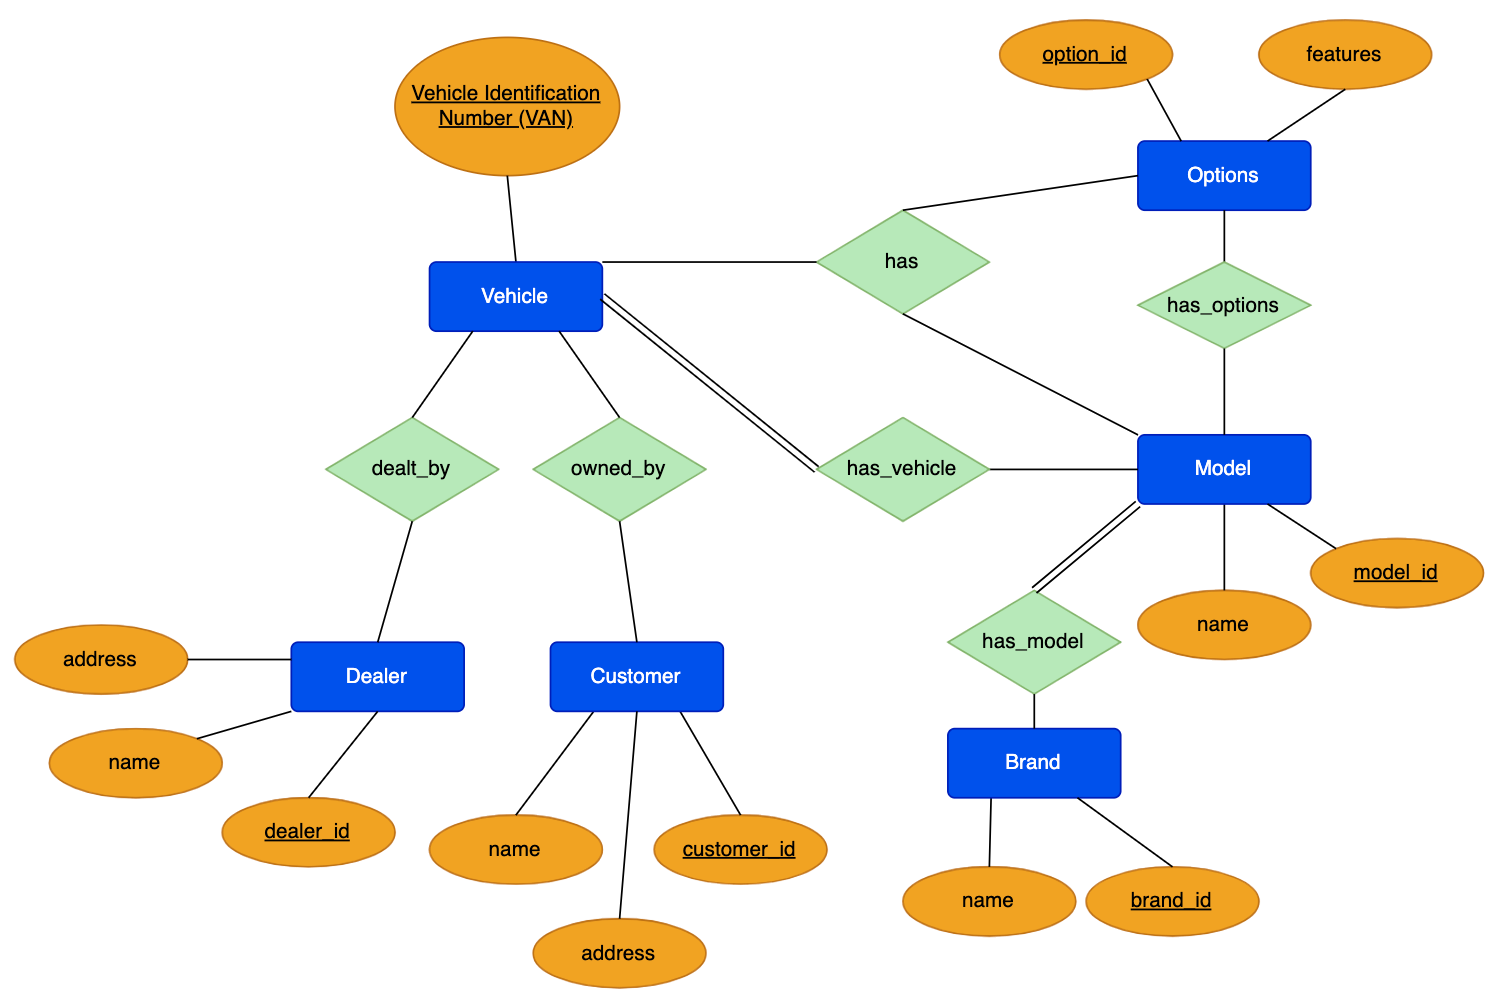
\includegraphics[scale=0.62]{screenshots/q1_screenshot.png}
    \label{fig:my_label1}
    \caption{E-R Diagram}
\end{figure}

\newpage

\subsubsection*{(b) Relational schemas}
\vspace{3mm} \\
\fbox{ 
    \begin{minipage}{40em}
    \inputminted{text}{problem1.txt}
    \end{minipage}
}
\vspace{5mm} \\
\textbf{Assumption:}
\begin{itemize}
    \item For handling the given conditon, i.e. each model can be offered with a variety of options, but an individual car may have only some (or none) of the available options we have made relationship \textbf{has\_vehicles} between Model and Vehicle, \textbf{has\_options} between Model and Options to ensure model has various options and \textbf{has} between Vehicle and (Options, Model) considering second quantity as single entity to make sure that individual car may have some available options.
    \item An alternate design could be made by connecting the has relation to an aggregated entity, formed by “joining” the tables of Model, has\_options, and Options. And then we would connect has only to vehicle and has\_options.
\end{itemize}

\newpage

\subsubsection*{(c) Table of constraints}

\begin{table}[!hbt]
    \centering
    \begin{tabular}{|c|c|c|c|c|} 
        \hline
        \textbf{Table} & \textbf{Primary Key} & \textbf{Domain of P.K.} & 
        \textbf{
        \begin{tabular}[c]{@{}c@{}}Foreign keys\\(Referencing table) \end{tabular}} & \textbf{Not Null} \\ 
        \hline\hline
c        Brand & brand\_id & VARCHAR & - & - \\ 
        \hline
        Model & model\_id & VARCHAR & - & - \\
        \hline
        Vehicle & VIN & VARCHAR & - & - \\
        \hline
        Options & option\_id & VARCHAR & - & - \\
        \hline
        Customer & customer\_id & VARCHAR & - & - \\
        \hline
        Dealer & dealer\_id & VARCHAR & - & - \\
        \hline
        has\_model & 
        \begin{tabular}[c]{@{}c@{}}model\_id \\ brand\_id \end{tabular} & 
        \begin{tabular}[c]{@{}c@{}}VARCHAR \\ VARCHAR \end{tabular} & 
        \begin{tabular}[c]{@{}c@{}}model\_id references Model\\brand\_id references Brand \end{tabular} 
        & - \\
        \hline
        has\_vehicle & 
        \begin{tabular}[c]{@{}c@{}}model\_id \\ VIN \end{tabular} & 
        \begin{tabular}[c]{@{}c@{}}VARCHAR \\ VARCHAR \end{tabular} & 
        \begin{tabular}[c]{@{}c@{}}model\_id references Model\\VIN references Vehicle \end{tabular} 
        & - \\
        \hline
        has\_options & 
        \begin{tabular}[c]{@{}c@{}}model\_id \\ option\_id \end{tabular} & 
        \begin{tabular}[c]{@{}c@{}}VARCHAR \\ VARCHAR \end{tabular} & 
        \begin{tabular}[c]{@{}c@{}}model\_id references Model\\option\_id references Options \end{tabular} 
        & - \\
        \hline
        has & 
        \begin{tabular}[c]{@{}c@{}}VIN \\ model\_id \\ option\_id \end{tabular} & 
        \begin{tabular}[c]{@{}c@{}}VARCHAR \\ VARCHAR \\ VARCHAR \end{tabular} & 
        \begin{tabular}[c]{@{}c@{}}VIN references Vehicle \\ (model\_id,option\_id) \\ references has\_options \end{tabular}
        & - \\
        \hline
        dealt\_by & 
        \begin{tabular}[c]{@{}c@{}}VIN \\ dealer\_id \end{tabular} & 
        \begin{tabular}[c]{@{}c@{}}VARCHAR \\ VARCHAR \end{tabular} & 
        \begin{tabular}[c]{@{}c@{}}VIN references Vehicle\\dealer\_id references Dealer \end{tabular} 
        & - \\
        \hline
        owned\_by & 
        \begin{tabular}[c]{@{}c@{}}VIN \\ customer\_id \end{tabular} & 
        \begin{tabular}[c]{@{}c@{}}VARCHAR \\ VARCHAR \end{tabular} & 
        \begin{tabular}[c]{@{}c@{}}VIN references Vehicle\\customer\_id references Customer \end{tabular} 
        & - \\
        \hline
        
    \end{tabular}
    \caption{Table of constraints}
    \label{tab:my_label}
\end{table}

\newpage
%---------------------------------------------------------------------

\section{Problem 2}

\subsection*{Design a database for a world-wide package delivery company (e.g., DHL or Fed EX).} 
\textbf{Given Information:} The database must be able to keep track of customers (who ship items) and customers (who receive items); some customers may do both. Each package must be identifiable and trackable, so the database must be able to store the location of the package and its history of locations. \\
Locations include trucks, planes, airports, and warehouses. Your design should include an E-R diagram, a set of relational schemas, and a list of constraints, including primary-key and foreign-key constraints. 

\subsubsection*{(a) E-R Diagram}

\begin{figure}[!hbt]
    \centering
    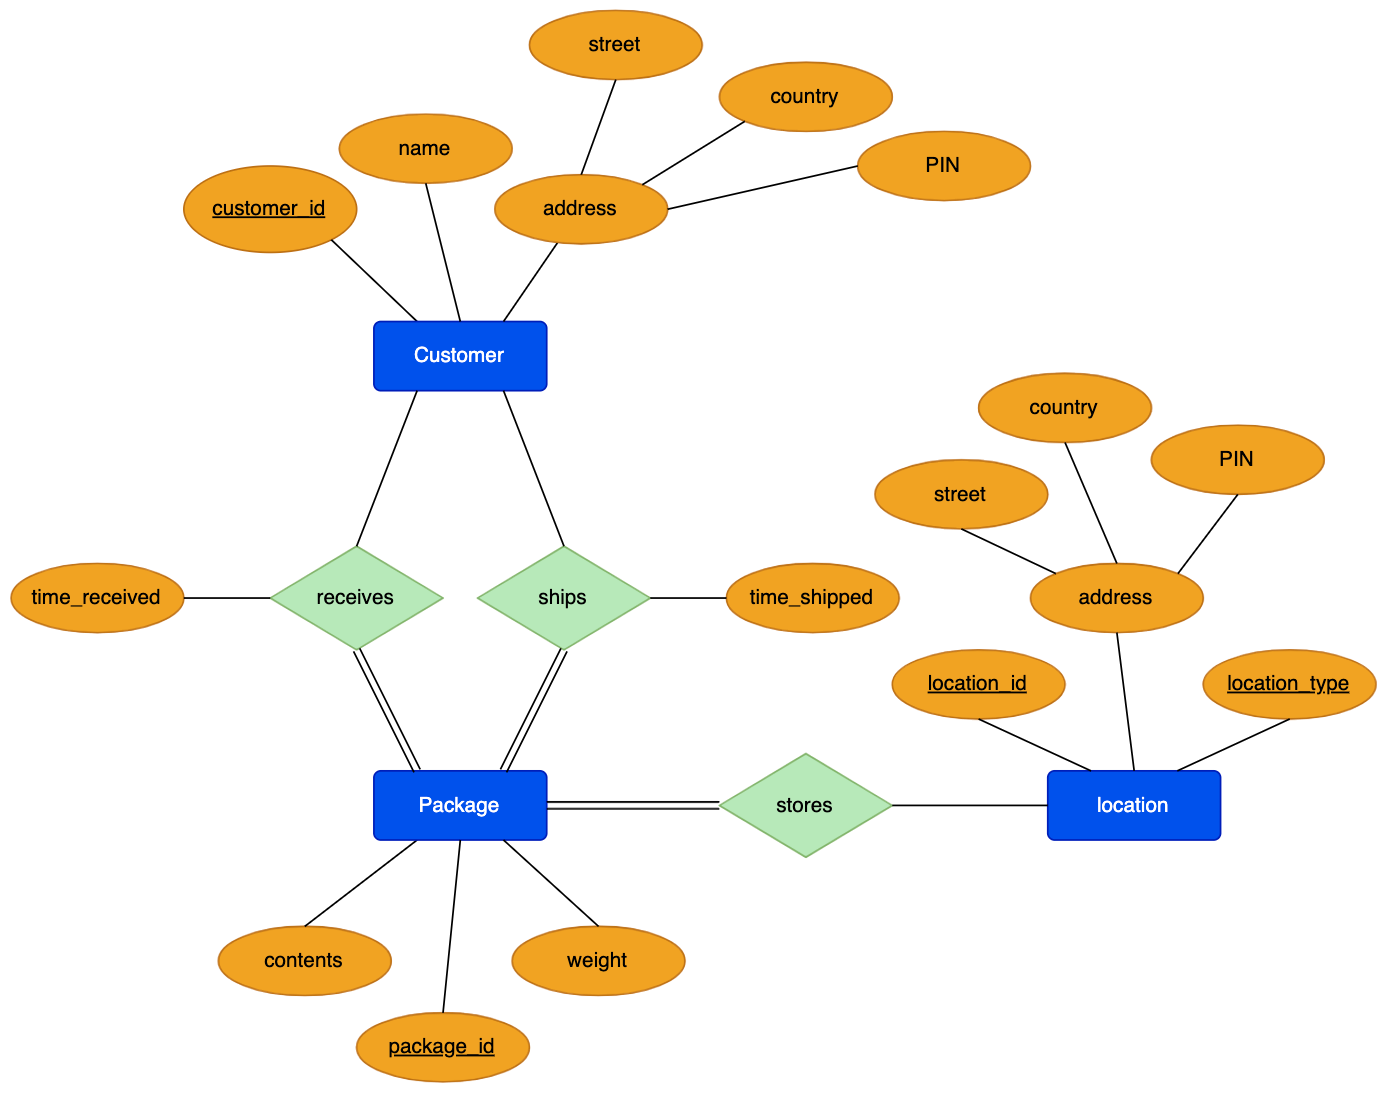
\includegraphics[scale=0.65]{screenshots/q2_screenshot.png}
    \label{fig:my_label1}
    \caption{E-R Diagram}
\end{figure}

\newpage

\subsubsection*{(b) Relational schemas}

\fbox{ 
    \begin{minipage}{40em}
    \inputminted{text}{problem2.txt}
    \end{minipage}
}
\vspace{2cm} \\
\textbf{Assumption:}
\begin{itemize}
    \item Here to handle the given condition, i.e. Locations include trucks, planes, airports, and warehouses, we made location\_id to identify each location history uniquely and location\_type to ensure we include trucks, planes, airports, and warehouses. We could have also ellaborated location\_type into futher subtypes such as transportation\_type and storage\_type. But here location\_type along with location\_id handles each case separately.
\end{itemize}

\newpage

\subsubsection*{(c) Table of constraints}

\begin{table}[!hbt]
    \centering
    \begin{tabular}{|c|c|c|c|c|} 
        \hline
        \textbf{Table} & \textbf{Primary Key} & \textbf{Domain of P.K.} & 
        \textbf{
        \begin{tabular}[c]{@{}c@{}}Foreign keys\\(Referencing table) \end{tabular}
        } & 
        \textbf{Not Null}\\ 
        \hline\hline
        Customer & customer\_id & VARCHAR & - & - \\ 
        \hline
        Package & package\_id & VARCHAR & - & - \\
        \hline
        Location & 
        \begin{tabular}[c]{@{}c@{}}location\_id \\ location\_type \end{tabular}
        & 
        \begin{tabular}[c]{@{}c@{}}VARCHAR \\ VARCHAR \end{tabular}
        & - & - \\
        \hline
        stores & 
        \begin{tabular}[c]{@{}c@{}}package\_id\\location\_id\\location\_type \end{tabular} & 
        \begin{tabular}[c]{@{}c@{}}VARCHAR\\ VARCHAR\\ VARCHAR \end{tabular} & 
        \begin{tabular}[c]{@{}c@{}}package\_id references Package\\location\_id references Location\\location\_type references Location \end{tabular} 
        & - \\
        \hline
        receives & 
        \begin{tabular}[c]{@{}c@{}}package\_id\\customer\_id\\time\_received \end{tabular} & 
        \begin{tabular}[c]{@{}c@{}}VARCHAR\\ VARCHAR\\ VARCHAR \end{tabular} & 
        \begin{tabular}[c]{@{}c@{}}package\_id references Package\\customer\_id references Customer \end{tabular} 
        & - \\
        \hline
        ships & 
        \begin{tabular}[c]{@{}c@{}}package\_id\\customer\_id\\time\_shipped \end{tabular} & 
        \begin{tabular}[c]{@{}c@{}}VARCHAR\\ VARCHAR\\ VARCHAR \end{tabular} & 
        \begin{tabular}[c]{@{}c@{}}package\_id references Package\\customer\_id references Customer \end{tabular} 
        & - \\
        \hline
    \end{tabular}
    \caption{Table of constraints}
    \label{tab:my_label}
\end{table}

\newpage

%---------------------------------------------------------------------------------

\section{Problem 3}

\subsection*{Find loophole in given web application scheme}
\onehalfspacing

\textbf{Question:} \\ 
Consider a carelessly written Web application for an online-shopping site, which 
stores the price of each item as a hidden form variable in the Web page sent to 
the customer; when the customer submits the form, the information from the hidden
form variable is used to compute the bill for the customer. What is the loophole 
in this scheme? (There was a real instance where the loophole was exploited by 
some customers of an online shopping site, before the problem was detected and 
fixed.) \\

\noindent
\textbf{Answer: } \\

A customer or hacker can anonymously edit the HTML source code of the 
Web page by right clicking on webpage and then selecting inspect 
option, and after this they can replace the value of the hidden 
variable price with whatever value they want, and thus they can use
the modified Web page to place an order. So the Web application
would then use the user-modified value as the price of the product.


Some times Customer can even buy the items for free if he changes the
price to zero. In any case, company will go in loss, it won't even 
know because of the loophole. To avoid this situation, they should 
use some encryption method for the form or they shouldn't send the 
price as an element in the form, instead they should set it from back-
end by default. 
 % Set line spacing to 1.5

\singlespacing 

\newpage
%---------------------------------------------------------------------

\section{Problem 4}

\onehalfspacing
\subsection*{Find risk in given web application scheme}

\textbf{Question:} \\ 
Consider another carelessly written Web application, which uses a servlet that checks if there was an active session, but does not check if the user is authorized to access that page, instead depending on the fact that a link to the page is shown only to authorized users. What is the risk with this scheme? (There was a real instance where applicants to a college admissions site could, after logging into the Web site, exploit this loophole and view information they were not authorized to see; the unauthorized access was however detected, and those who accessed the information were punished by being denied admission.) \\

\noindent
\textbf{Answer: } \\ 
There is a concept known as web proxy logs, their main purpose is to relay URL requests from clients to a server, receive the responses from the server and send them back to the appropriate clients.The web proxy acts as a gateway between the Internet and browsers on a local network. Thus, analysing web proxy
logs can give unobtrusive insights to the browsing behavior of computer
users and provide an overview of the Internet usage in an organization. So there is risk of web proxies happening here. 

Here, even if the link to the page is shown only to authorized users,
an unauthorized user may somehow come to know of the existence of the
link (for example, from an unauthorized user, or via Web proxy logs). The
user may then login to the system, and access the unauthorized page by
entering its URL in the browser. If the check for user authorization was
unintentionally left out from that page, the user will be able to see the result
of the page. So the user can use that unauthorized data somewhere else, and in turn it may have bad effect on the organization or company. 

Solution for that is to use The HTTP referer attribute to block a naive attempt to exploit such loopholes, by ensuring the referer value is from a valid page of the web site. However, the referer attribute is set by the browser, and can be spoofed, so a malicious user can easily work around the referer check.

\singlespacing 
\newpage
%---------------------------------------------------------------------

\section{Problem 5}
\setstretch{1.2}
\subsection*{Explain how the protocol might use digital certificates to verify authenticity of the site.}

\textbf{Question:} \\ 
Hackers may be able to fool you into believing that their Web site is actually a Web site (such as a bank or credit card Web site) that you trust. This may be done by misleading email, or even by breaking into the network infrastructure and rerouting network traffic destined for, say mybank.com, to the hacker’s site. If you enter your user name and password on the hacker’s site, the site can record it, and use it later to break into your account at the real site. When you use a URL such as https://mybank.com , the HTTPS protocol is used to prevent such attacks. Explain how the protocol might use digital certificates to verify authenticity of the site. \\

\noindent
\textbf{Answer: } \\ 
Authentication can be handled by a system of digital certificates, whereby public keys are signed by a certification agency, whose public key is well known. For example, the public keys of the root certification authorities are stored in standard Web browsers. A certificate issued by them can be verified by using the stored public keys.

Digital certificates are widely used to authenticate Web sites to users, to prevent malicious sites from masquerading as other Web sites. In the HTTPS protocol (the secure version of the HTTP protocol), the site provides its digital certificate to the browser, which then displays it to the user. If the user accepts the certificate, the browser then uses the provided public key to encrypt data. A malicious site will have access to the certificate, but not the private key, and will thus not be able to decrypt the data sent by the browser. Only the authentic site, which has the corresponding private key, can decrypt the data sent by the browser. We note that public-/private-key encryption and decryption costs are much higher than encryption/decryption costs using symmetric private keys. To reduce encryption costs, HTTPS actually creates a one-time symmetric key after authentication, and uses it to encrypt data for the rest of the session.

Digital certificates can also be used for authenticating users. The user must submit a digital certificate containing her public key to a site, which verifies that the certificate has been signed by a trusted authority. The user’s public key can then be used in a challenge–response system to ensure that the user possesses the corresponding private key, thereby authenticating the user.

\singlespacing
\newpage
%---------------------------------------------------------------------

\section{Problem 6}

\subsection*{ Write a servlet and associated HTML code for the following simple application: A user logins using userid and password and then a servlet authenticates the user (based on user ids and passwords stored in a database relation), and sets a session variable called userid after authentication}


\subsection{Query}
The q6.sql file contents are shown here.
\vspace{5mm} \\
\fbox{ 
    \begin{minipage}{40em}
    \inputminted{mysql}{src/q6.sql}
    \end{minipage}
}

\newpage

The Login.jsp file contents are shown here.
\vspace{5mm} \\
\fbox{ 
    \begin{minipage}{40em}
    \inputminted{jsp}{src/Login1.txt}
    \end{minipage}
} 

\newpage

\fbox{ 
    \begin{minipage}{40em}
    \inputminted{jsp}{src/Login2.txt}
    \end{minipage}
}

\newpage

The Result.jsp file contents are shown here.
\vspace{5mm} \\
\fbox{ 
    \begin{minipage}{40em}
    \inputminted{jsp}{src/Result.txt}
    \end{minipage}
}

\newpage

The ResultException.jsp file contents are shown here
\vspace{5mm} \\
\fbox{ 
    \begin{minipage}{40em}
    \inputminted{jsp}{src/ResultException.txt}
    \end{minipage}
}

\newpage

The LoginServlet.java file contents are shown here
\vspace{5mm} \\
\fbox{ 
    \begin{minipage}{40em}
    \inputminted{java}{src/LoginServlet1.txt}
    \end{minipage}
}

\newpage

\fbox{ 
    \begin{minipage}{40em}
    \inputminted{java}{src/LoginServlet2.txt}
    \end{minipage}
}

\newpage

\subsection{Screenshots}

All the cases are handled in following screenshots: 
\begin{itemize}
    \item All the inserted data for userid and password by using sql file is displayed in the figure \ref{fig:data}.
    \item Logging in with correct credentials.
    \item Logging in with in-correct credentials.
\end{itemize}

\vspace{5mm}
\begin{figure}[!hbt]
    \centering
    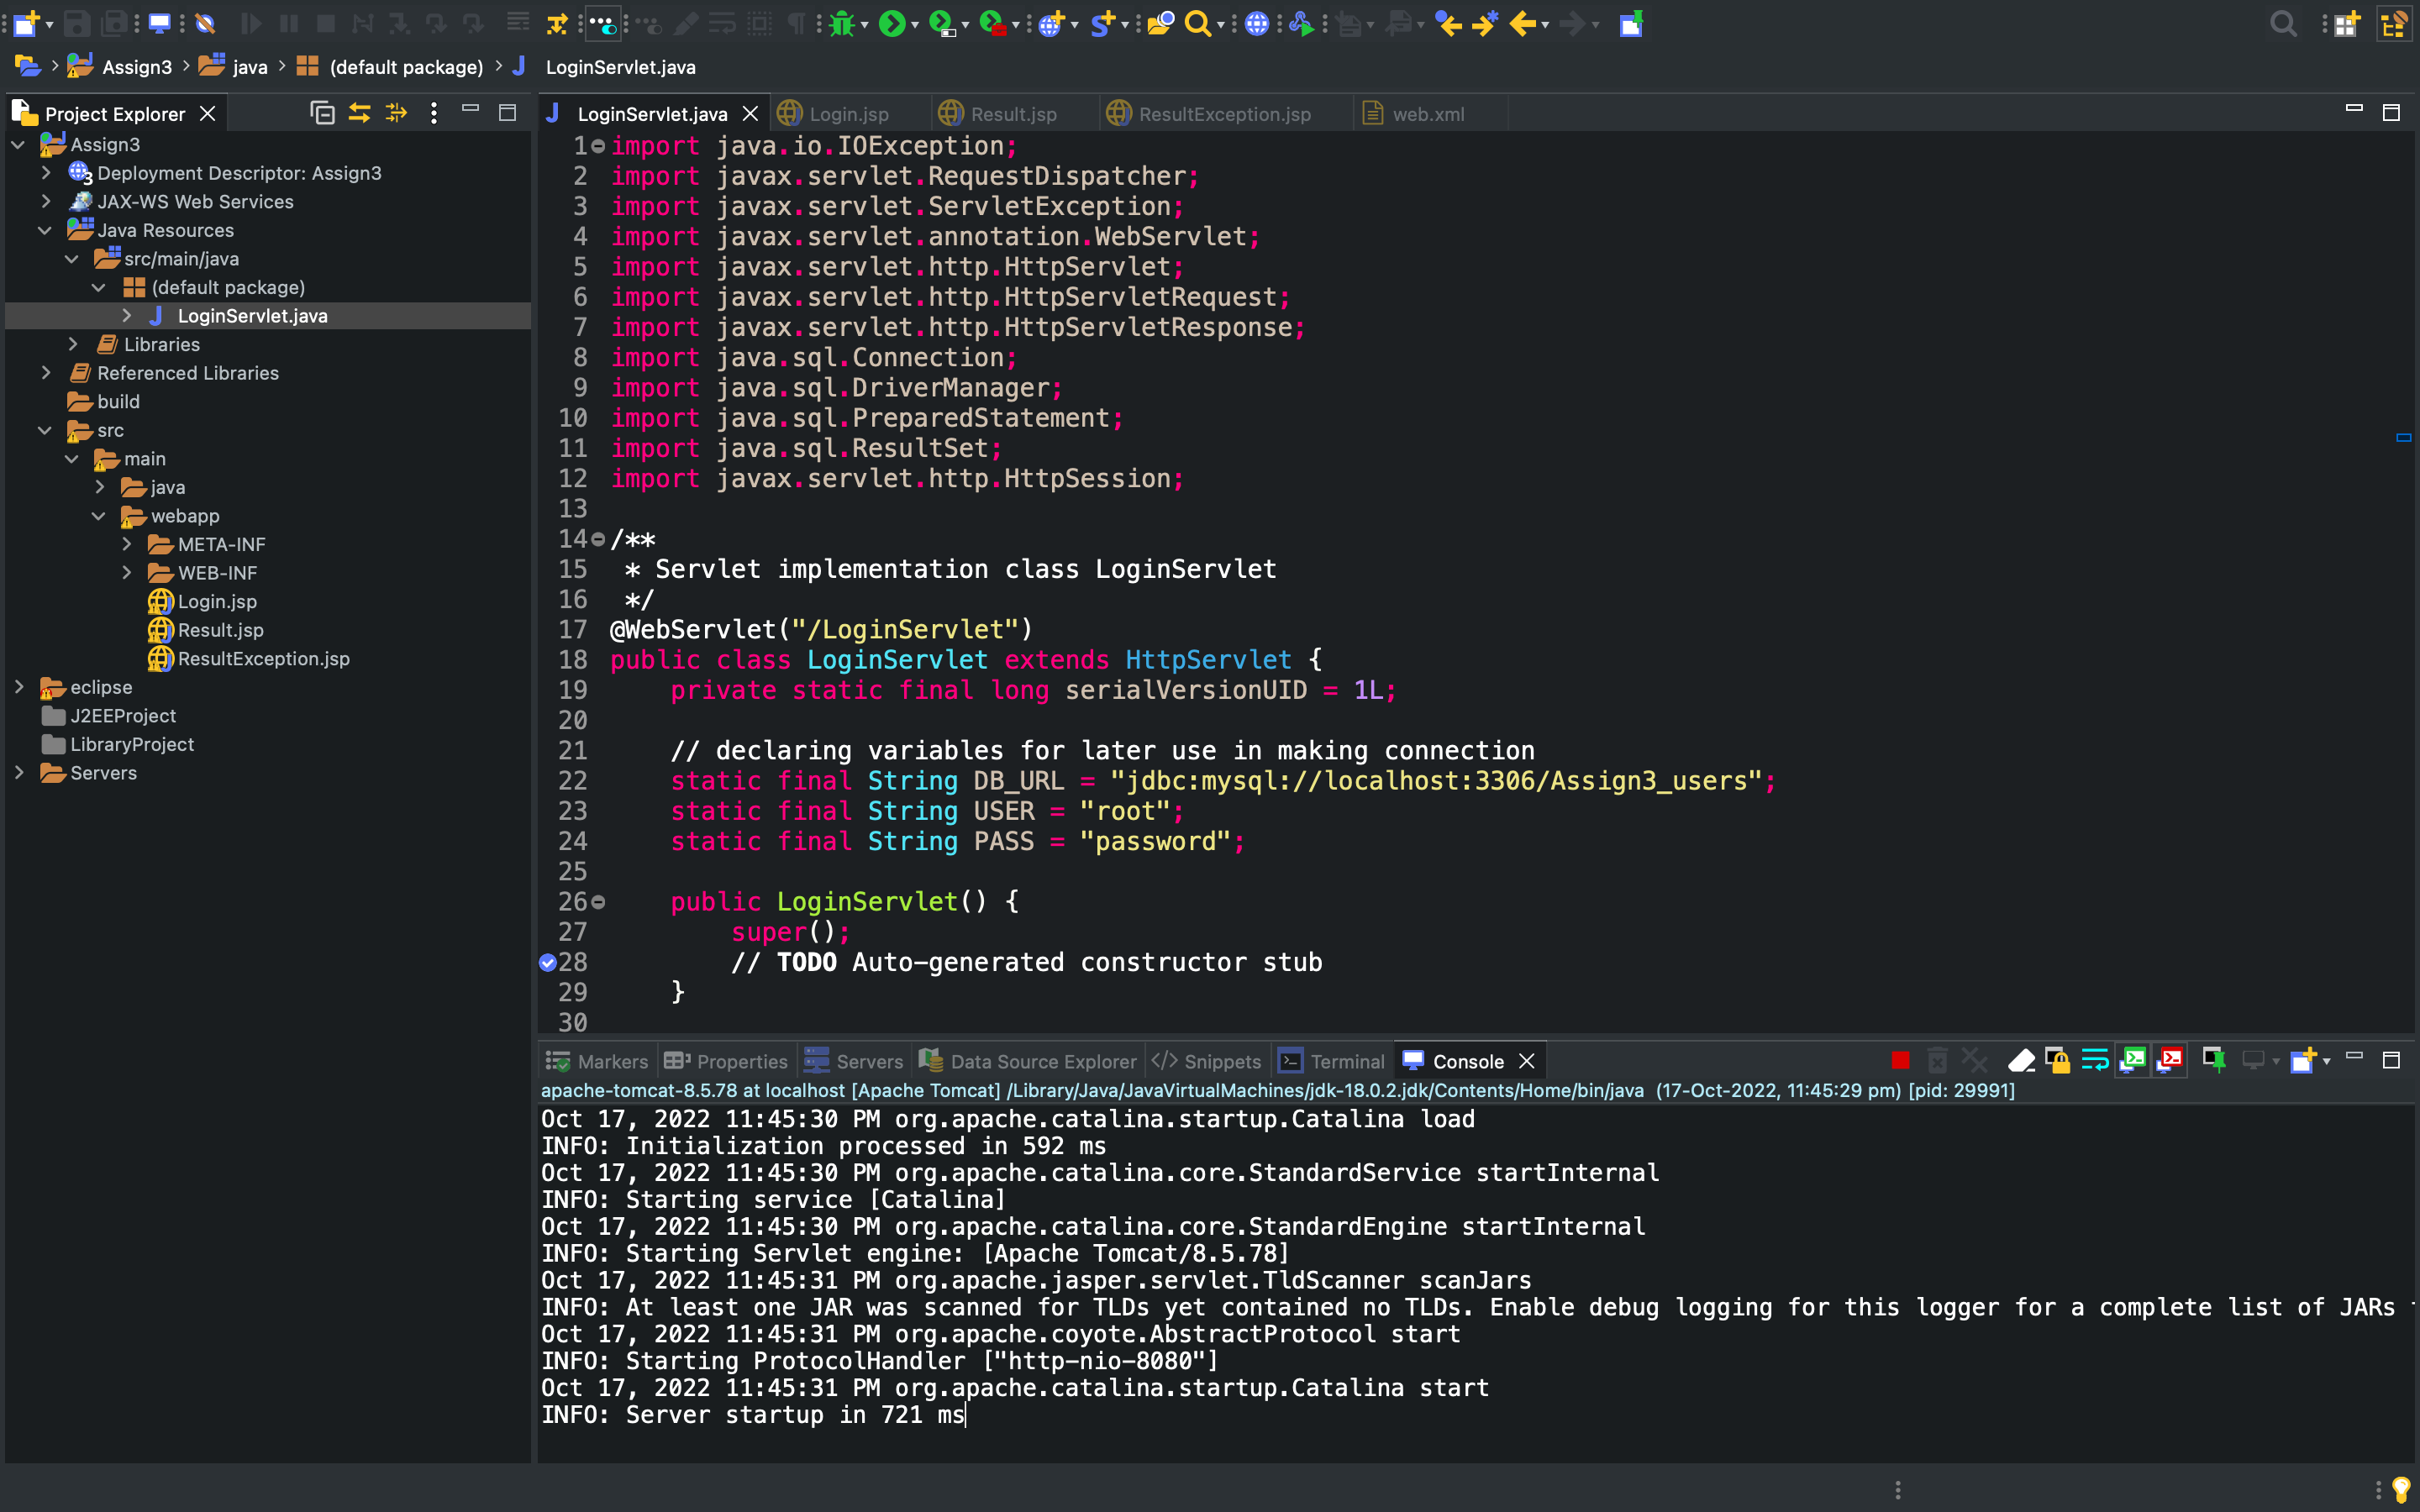
\includegraphics[scale=0.35]{screenshots/1.png}
    \label{fig:my_label1}
    \caption{IDE Screenshot with running server}
\end{figure}

\newpage

\begin{figure}[!hbt]
    \centering
    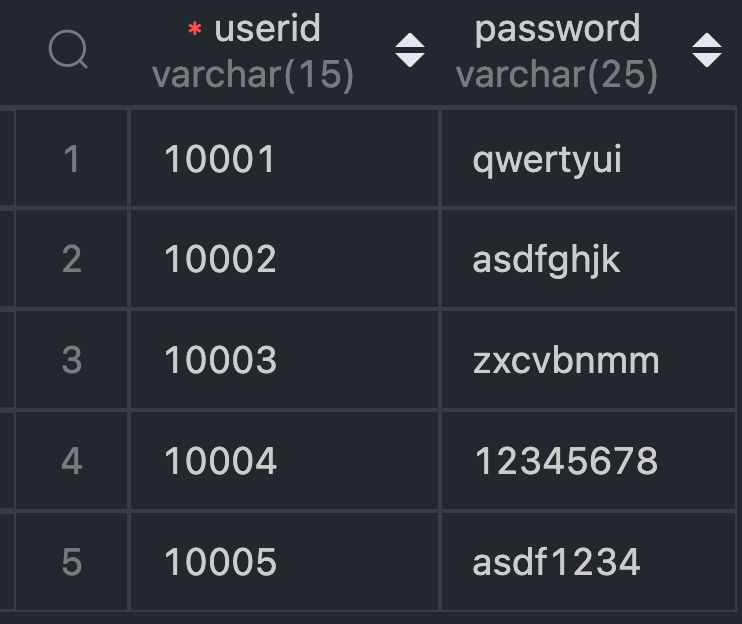
\includegraphics[scale=0.6]{screenshots/2.png}
    \label{fig:data}
    \caption{Data present inside \texttt{users} table}
\end{figure}

\begin{figure}[!hbt]
    \centering
    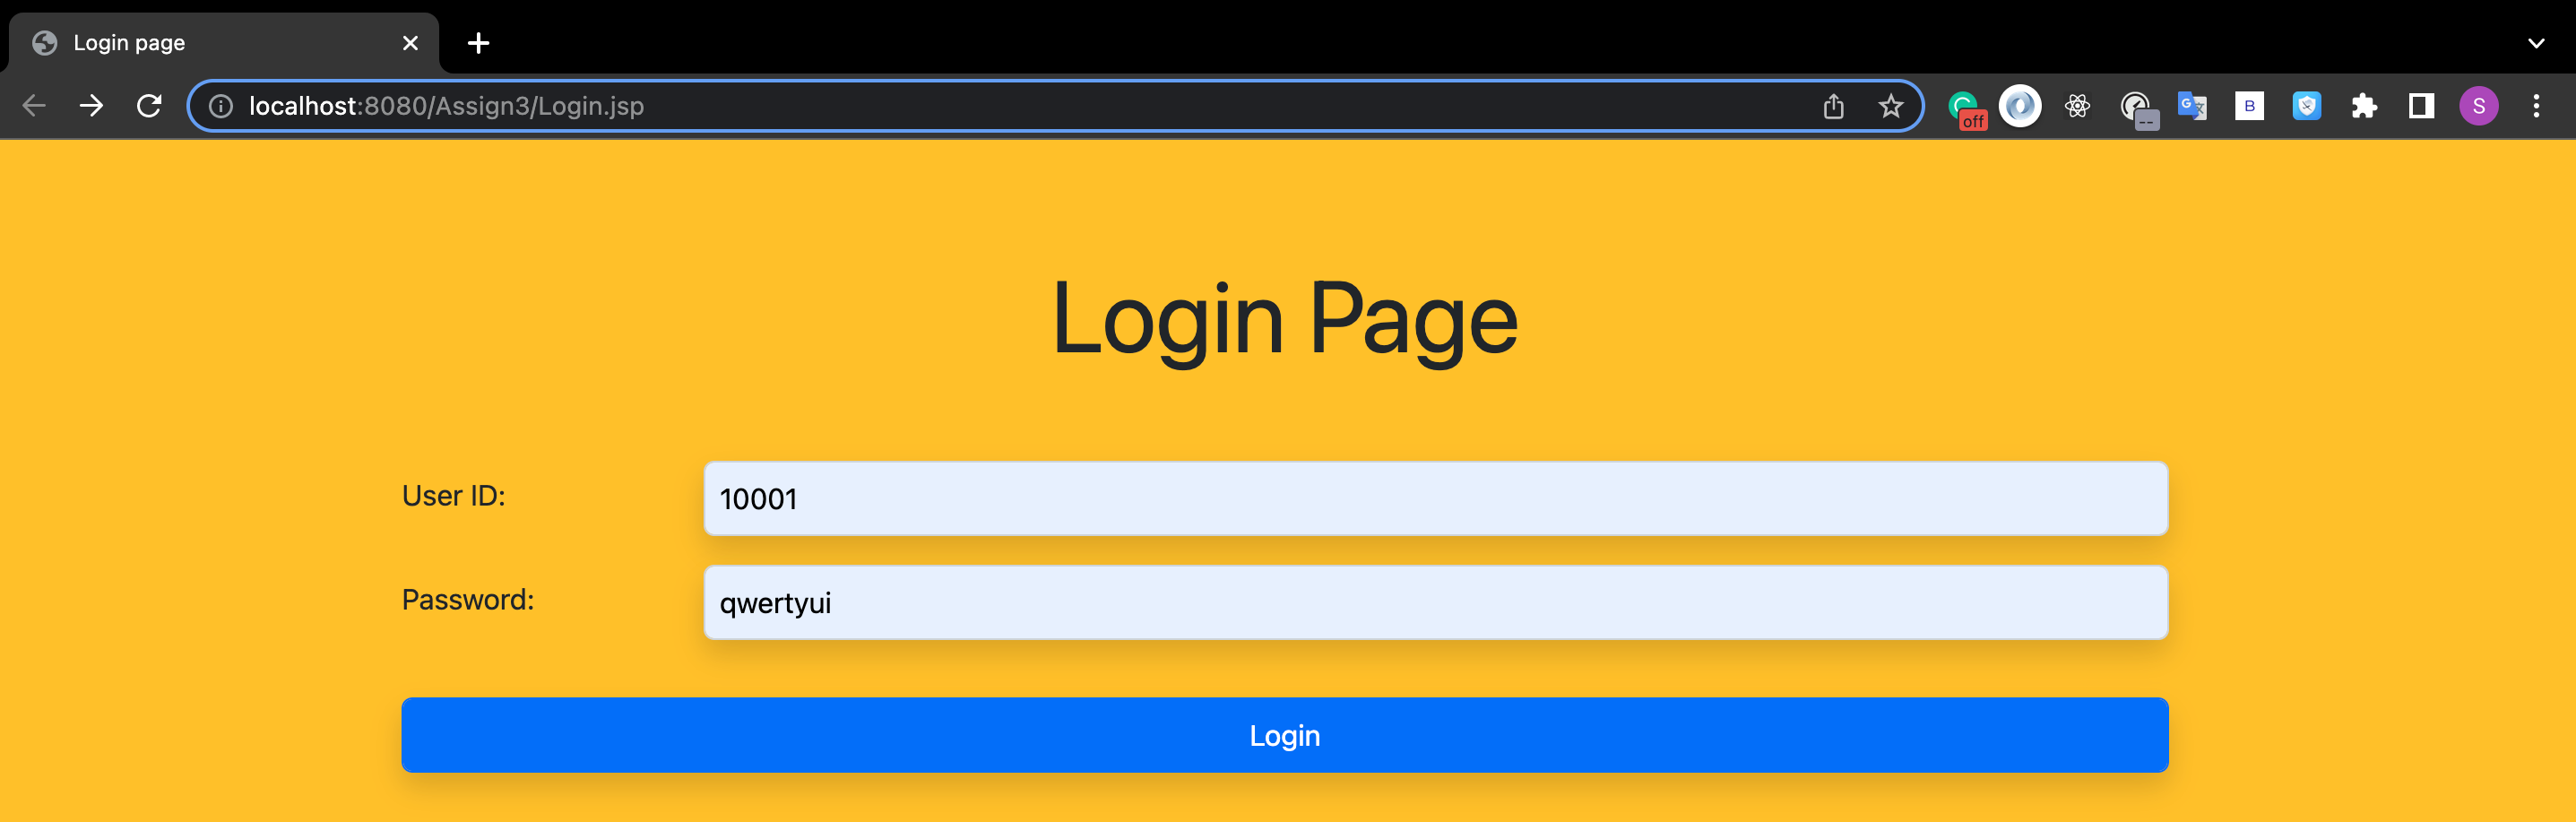
\includegraphics[scale=0.35]{screenshots/3.png}
    \label{fig:my_label1}
    \caption{Logging in with correct credentials}
\end{figure}

\begin{figure}[!hbt]
    \centering
    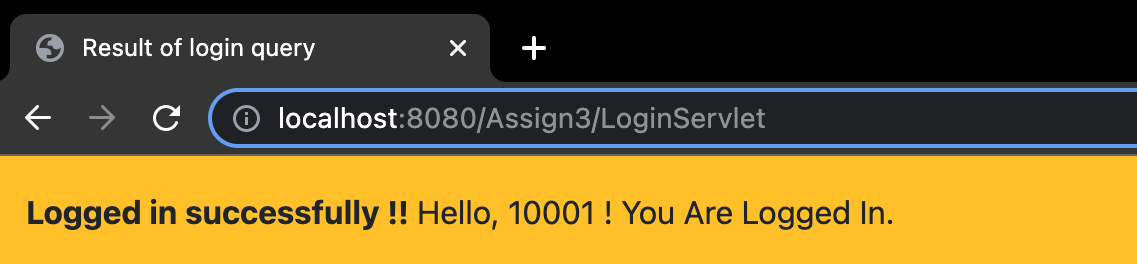
\includegraphics[scale=0.75]{screenshots/4.png}
    \label{fig:my_label1}
    \caption{Result of correct input and displaying session variable}
\end{figure}

\newpage

\begin{figure}[!hbt]
    \centering
    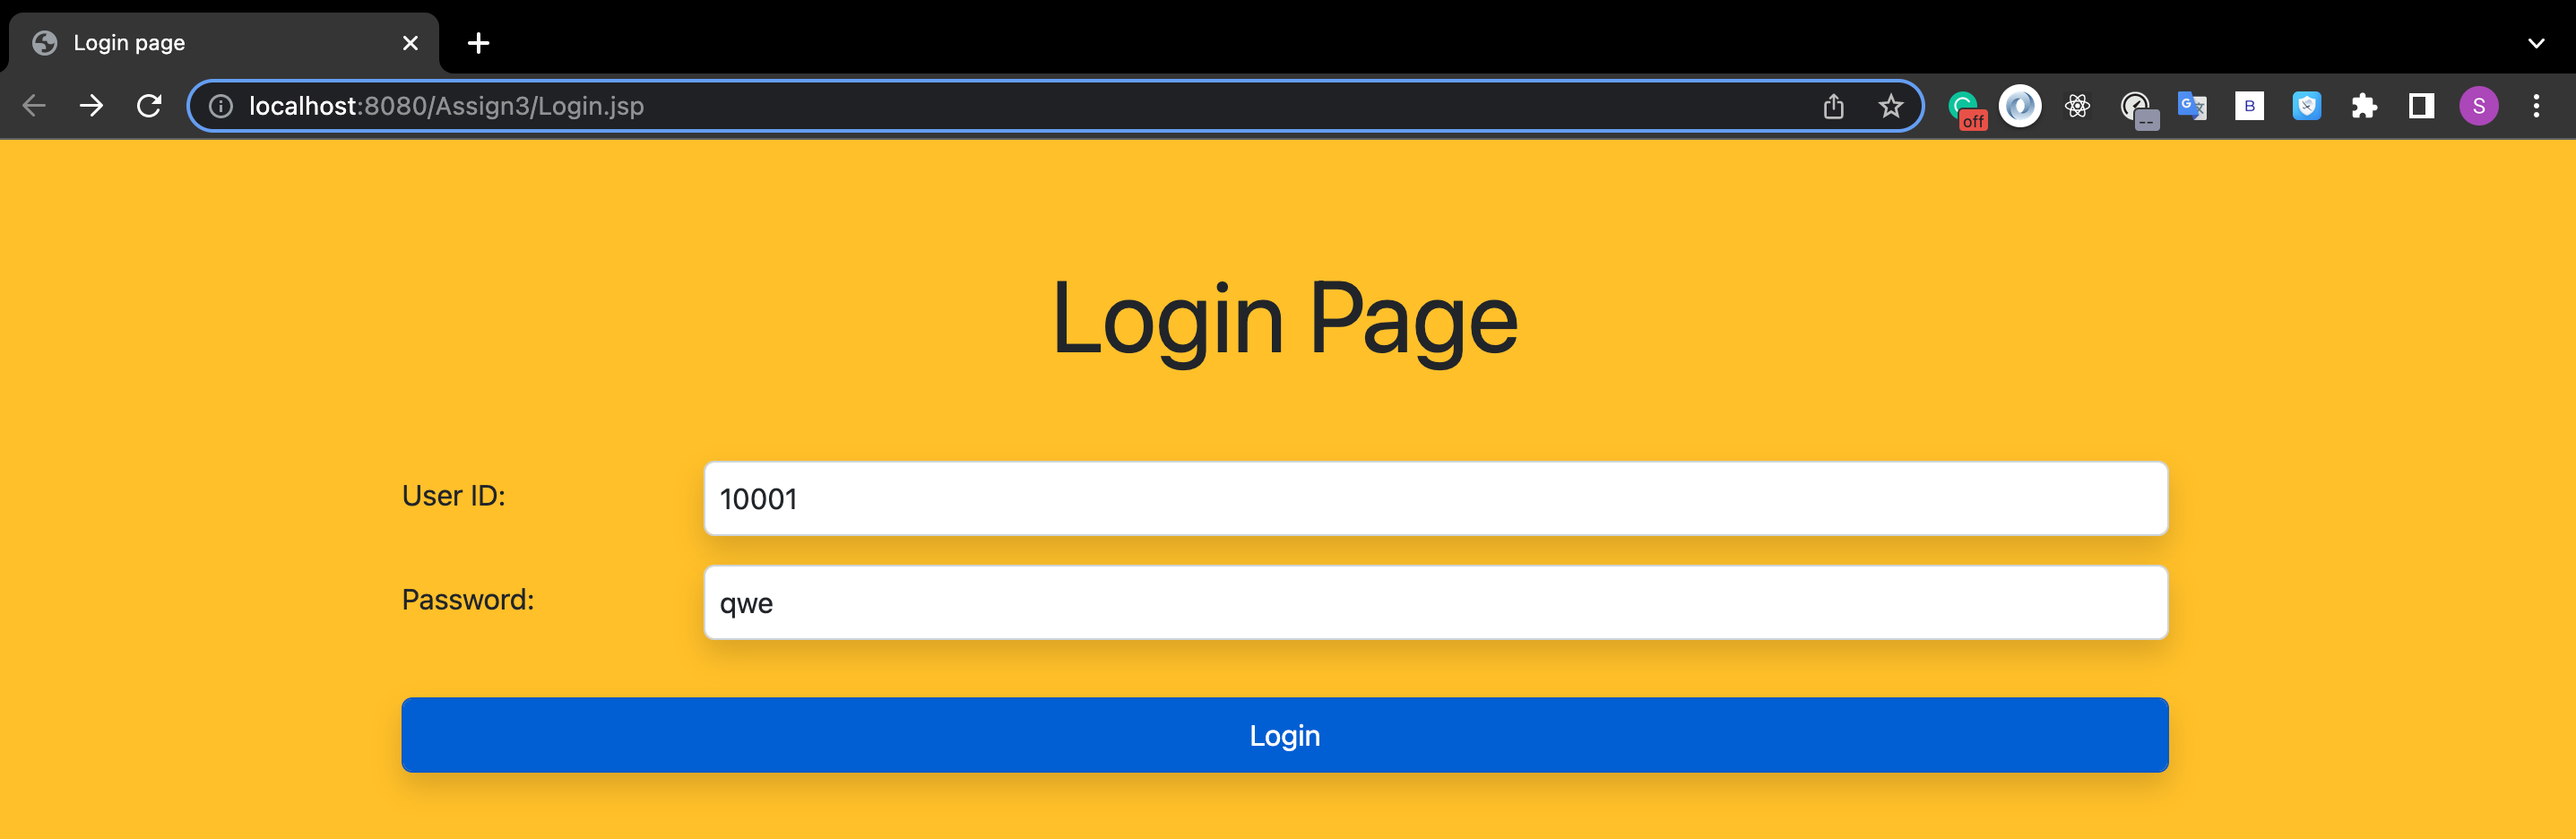
\includegraphics[scale=0.35]{screenshots/5.png}
    \label{fig:my_label1}
    \caption{Logging in with incorrect credentials}
\end{figure}

\vspace{2cm} 

\begin{figure}[!hbt]
    \centering
    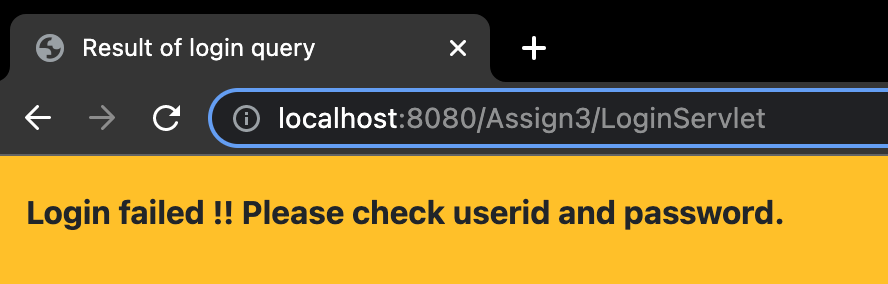
\includegraphics[scale=0.75]{screenshots/6.png}
    \label{fig:my_label1}
    \caption{Result of incorrect input}
\end{figure}

\newpage
%--------------------------------------------------------------

\section{Problem 7}

\subsection*{XSS Attack}
\setstretch{1.125}
\textbf{Question:} \\ 
What is an XSS attack? Explain how it works, and what measures must be taken to detect or prevent XSS attacks?
\\

\noindent
\textbf{Answer: } \\ 
A Web site that allows users to enter text, such as a comment or a name, and then stores it and later displays it to other users, is potentially vulnerable to a kind of attack called a cross-site scripting (XSS) attack. In such attack, when a different user views the entered text, the browser would execute the script, which can carry out actions such as sending private cookie information back to the malicious user, or even executing an action on a different Web server that the user may be logged into.

We can take an example of bank website. Lets say that user logins to his bank account at the time the script executes. Then that script is able to send cookie information regarding his bank account login back to the malicious user, who could use the information to connect to the bank’s Web server and may fool everyone to believe that the connection is from the original user.

Cross-site scripting (XSS) attack can be done in other ways also, like tempting a user into visiting a Web site that has malicious scripts embedded in its pages. Thus user gets caught in hacker's trap, and hacker gets the access to his data. 

To avoid such attacks following things can be done:
\begin{enumerate}
    \item Prevent your Web site from being used to launch XSS or XSRF attacks: \\
        This can be achieved by avoid taking text inputs from the users. We can also use functions that detect, or strip all such tags. These functions can be used to prevent HTML tags, and as a result, any scripts, from being displayed to the other users.
    
    \item Protect your Web site from XSS or XSRF attacks launched from other sites: \\
        If user log into to our web site and then he visits different web site  vulnerable to XSS, then in such case the malicious code executing on the user’s browser could execute actions on our Web site and can have access to session information related to our site. So some methods are there to prevent this.
        First being to check if the referer generated by HTTP protocol is valid. Second solution can be instead of using only the cookie to identify a session, the session could also be restricted to the IP address from which it was originally authenticated. Another solution could be to never use a GET method to perform any updates. 
\end{enumerate}
\singlespacing

\end{document}